\documentclass[a4paper,12pt]{article}
\usepackage[utf8]{inputenc}
\usepackage{graphicx}
\usepackage{graphics}
\usepackage{hyperref}
\usepackage{geometry}
\usepackage{float}
% \usepackage{comment}
\usepackage{tabularx}
\usepackage{booktabs}

%\usepackage{indentfirst}

\graphicspath{ {build/} } 
\geometry{left=2cm, right=2cm, top=2cm, bottom=2cm}

\begin{document}

\begin{titlepage}
    \begin{center}
        \vspace*{3cm}
        
        {\Huge \textbf{Laboratorio 2 - Grupo 7}}\\[1cm]
        {\LARGE Panel solar automático:\\ [0.5cm]  Selección de Hardware, Diagrama de bloques, periféricos, comunicaciones.}\\[2cm]
        
        \vfill
        
        {\Large \textbf{Integrantes }}\\[.5cm]
        \large
        \begin{tabular}{c c}
            Gartner, Francisco Nehuen & 69864/6 \\
            Marchesotti, Guido Daniel & 69923/9 \\
            Rosa, Fausto Pablo & 69843/1 \\
        \end{tabular}
        
        \vspace{1cm}
        
        \begin{figure}[b]
            \centering
            
\includegraphics[width=1\linewidth]{LOGOSFI-UNLP-color-01.png}
        \end{figure}
        
        %%{\large \today}
    \end{center}
\end{titlepage}

%%\newpage
%%\tableofcontents
%%\newpage

\section{Introducción}
En esta entrega se presentan los componentes necesarios para el desarrollo del proyecto \textbf{Panel Solar Automático}. En este documento encontrará las funciones que cumplirán dichos componentes así como las las características y criterios tomados en cuenta para su elección.
\section{Listado de componentes}
Los componentes necesarios serán los siguientes: 
\begin{itemize}
\item Microcontrolador
\item Sensor de Potencia
\item Sensor de Luz
\item Motores
\item Panel Solar
\item Regulador de Carga
\item Batería
\item Transmisor inalámbrico
\end{itemize}

En \hyperref[fig:diagrama]{figura 1} se puede observar un diagrama de bloques con su conexionado. 

\begin{figure}[H]
    \centering
    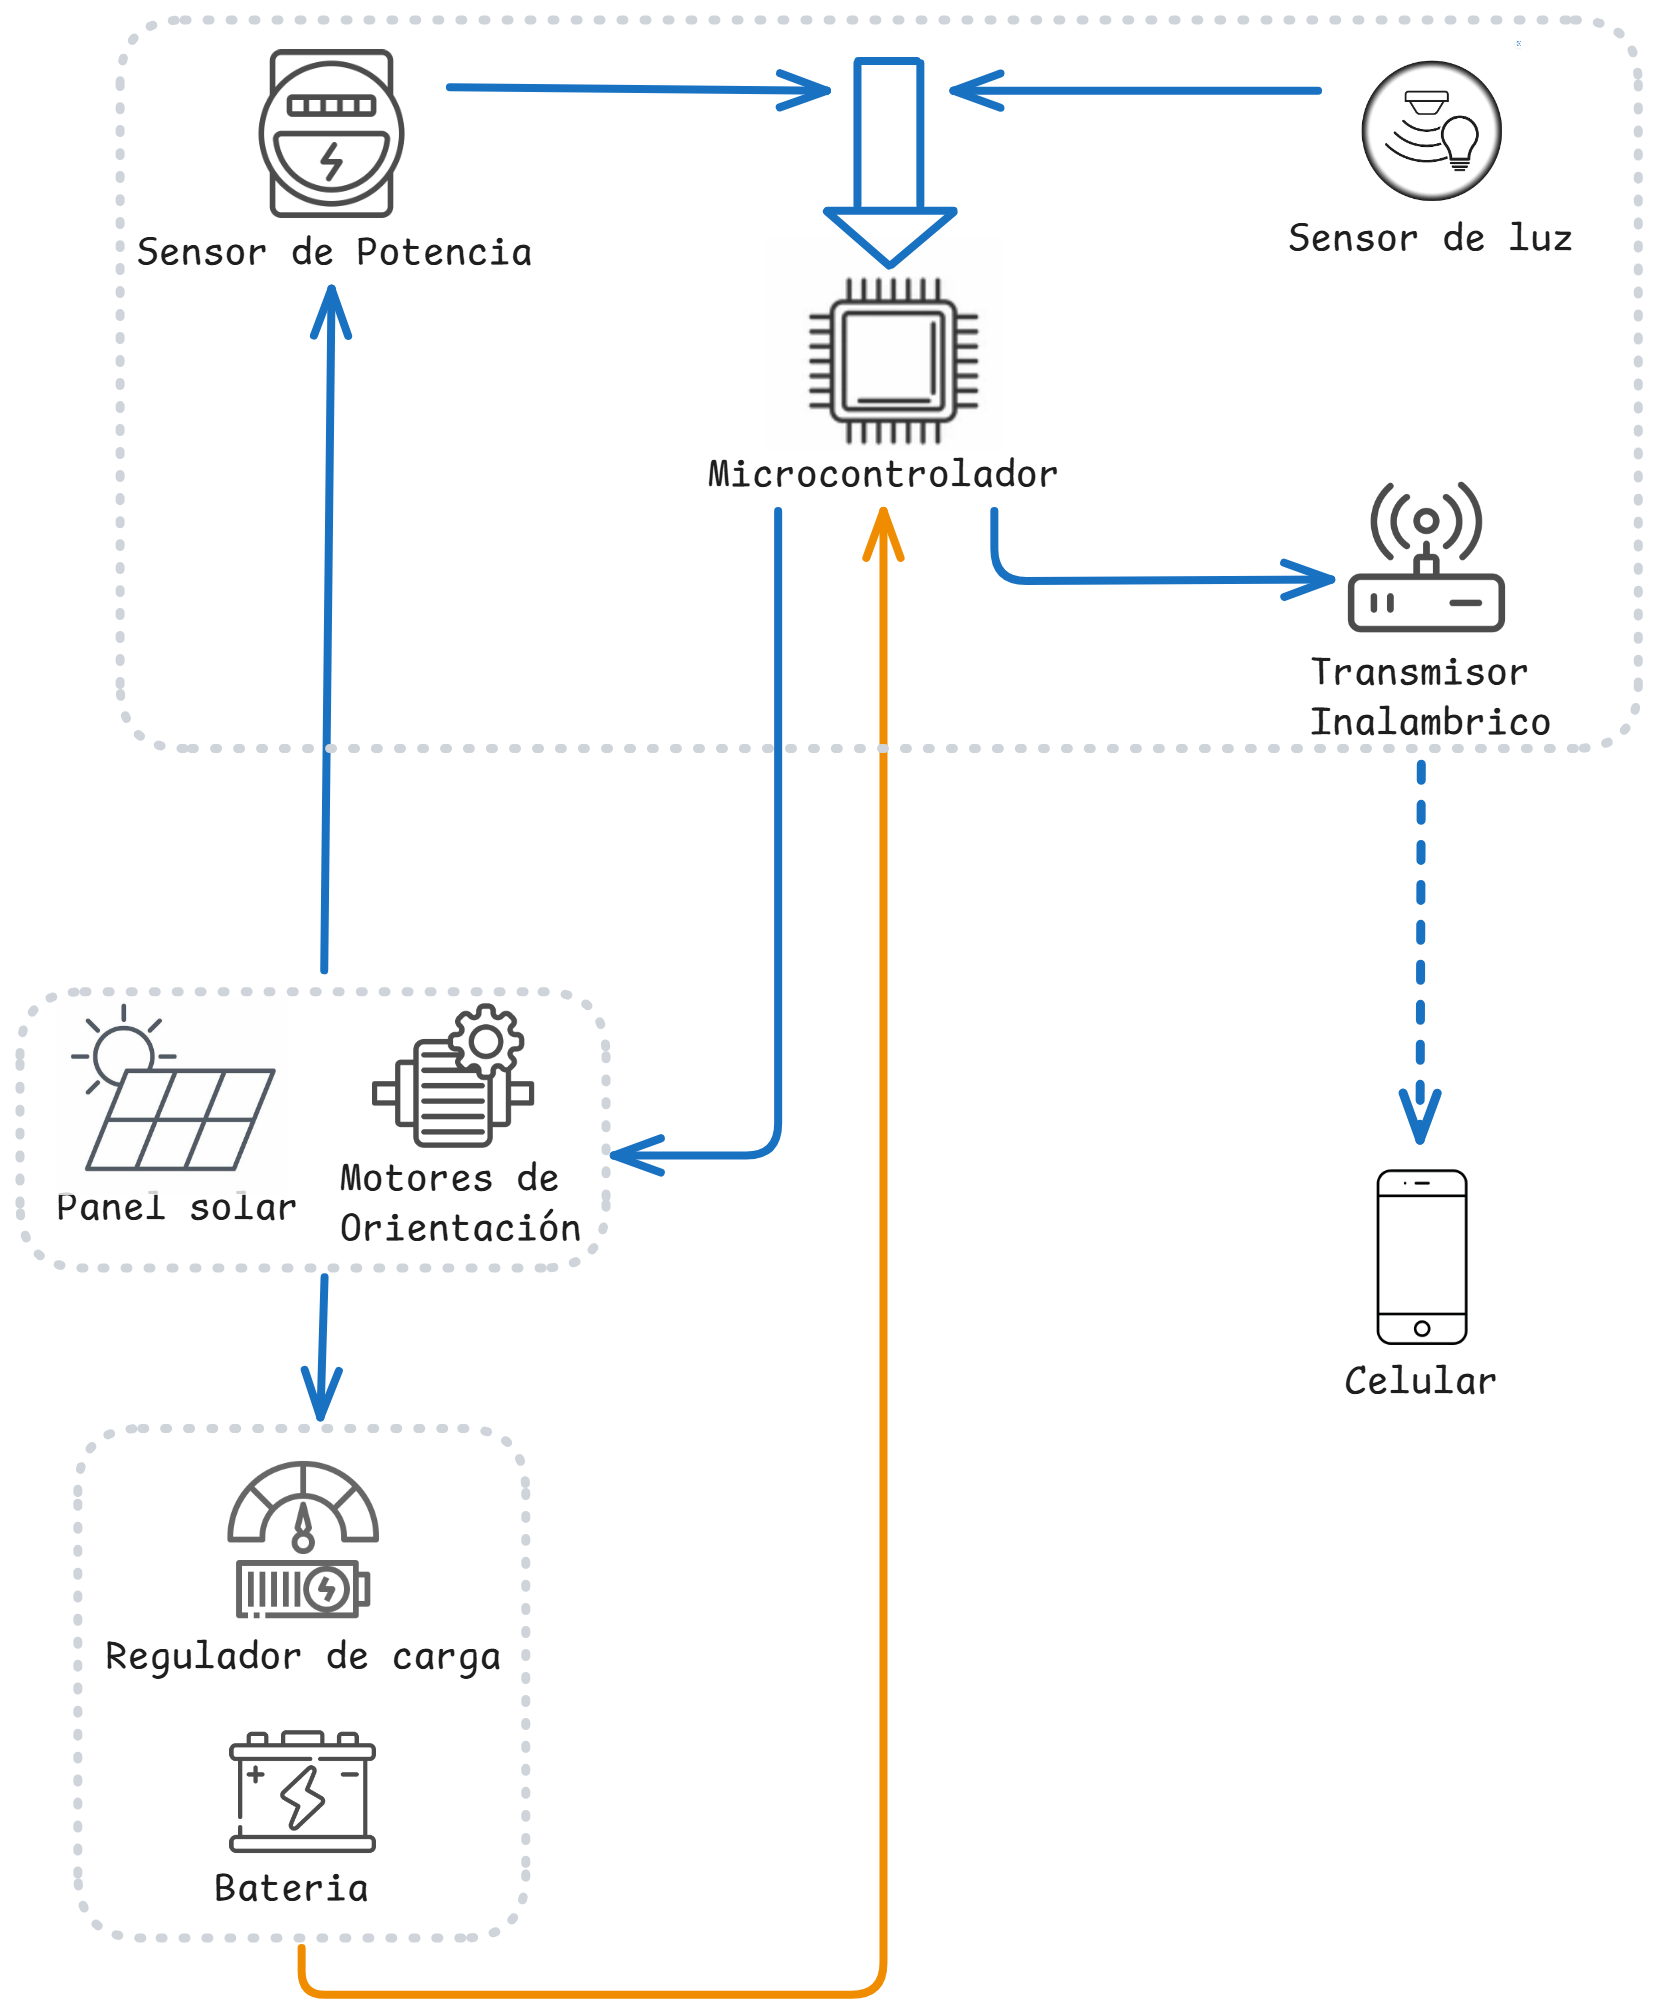
\includegraphics[width=0.75\linewidth]{diagrama_proyecto.png}
    \caption{ diagrama de bloques de los componentes generales}
    \label{fig:diagrama}
\end{figure}

\section{Análisis}
A continuación, se desarrollan las criterios tenidos en cuenta para cada uno de los componentes listados, teniendo en cuenta su función y requerimientos necesarios. Cabe aclarar que en la selección de todos los componentes se tuvo en cuenta la disponibilidad y el precio siendo estas importantes limitaciones en el desarrollo del trabajo practico.

\subsection{Microcontrolador}
Dentro del proyecto tenemos limitaciones impuestas para la elección del microcontrolador. Aún así, se pueden nombrar algunas características destacables del mismo que se ajustan a las tareas a realizar. Como el sistema de seguimiento solar no requiere una acción de control rápida, la transmisión de datos no requiere de una velocidad elevada y los cálculos a realizar son de bajo consto computacional, se puede elegir un microcontrolador de características moderadas. Esto nos permitirá disminuir el consumo de energía alcanzando un mayor eficiencia energética, característica importante en sistemas  dependientes de baterías. Además, el Atmega328p es un microcontrolador popular con amplias librerías ya desarrolladas y funcionales, facilitando el desarrollo con el mismo y su debuggeo.\\

\begin{table}[h!]
\centering
\begin{tabularx}{\textwidth}{l c *{3}{>{\centering\arraybackslash}X}}
\toprule
\textbf{Criterio} & \textbf{Ponderación (\%)} & \textbf{Atmega328p} & \textbf{Esp32} & \textbf{FPGA} \\
\midrule
C1: Costo           & 30\% &  1  &  1   &   -1  \\
C2: Disponibilidad & 30\% &  1    &  1   &  0   \\
C3: Practicidad & 10\% & 1    &  1   &   0  \\
%C4: Consumo   & 20\% &     &     &     \\
C4: Consumo  & 30\% &  1   &  0   &  0   \\
\midrule
\textbf{Total}           & 100\% &  4   &   3  &  -1   \\
\textbf{Total ponderado} &        &  100\%   &  70\%   & -30\%    \\
\textbf{Prioridad}       &        &  1   &  2   &   3  \\
\bottomrule
\end{tabularx}
\caption{Matriz de Pugh con ponderación por criterio}
\end{table}
Teniendo en cuenta la experiencia previa de los desarrolladores con las diferentes arquitecturas expuestas, se decide por el Atmega328p. Además de su bajo costo, consumo y por la imposición de la cátedra. 
\subsection{Sensor de Potencia}
Considerando las características del panel solar, se filtrara al componente en función de que sea capaz de operar dentro del rango esperado de potencia, corriente y tensión que entregara el panel solar. Se priorizaran criterios como la sencillez de uso, optando por componentes capaces de sensar múltiples variables. Valorando también apartados como la precisión y el consumo.
Debido a la lenta variación de la potencia, no se ha priorizado en la velocidad de muestreo a la hora de barajar entre los posibles componentes.\\ 

%INA 219 1\%\\ 
%Modulo Sensor Tension Corriente Max471 Para Arduino Emakers\\ 2\%
%Sensor Corriente Shunt 3ch Ina3221 Smbus I2c Itytarg\\ 1\%
%acs712\\

\begin{table}[h!]
\centering
\begin{tabularx}{\textwidth}{l c *{3}{>{\centering\arraybackslash}X}}
\toprule
\textbf{Criterio} & \textbf{Ponderación (\%)} & \textbf{INA 219} & \textbf{Max471} & \textbf{Ina3221} \\
\midrule
C1: Costo           & 40\% &  1  &  0   &   -1  \\
C2: Disponibilidad & 30\% &  1    &  1   &  1   \\
C3: Practicidad & 15\% & 1    &  0   &   1  \\
%C4: Consumo   & 20\% &     &     &     \\
C4: Precisión  & 15\% &  0   &  -1   &  1   \\
\midrule
\textbf{Total}           & 100\% &  3   &   0  &  2   \\
\textbf{Total ponderado} &        &  85\%   &  15\%   & 20\%    \\
\textbf{Prioridad}       &        &  1   &  3   &   2  \\
\bottomrule
\end{tabularx}
\caption{Matriz de Pugh con ponderación por criterio}
\end{table}

De los modulos expuestos, los INA usan protocolo I2C, siendo un protocolo ya antes utilizado por los desarrolladores. Se decide por el INA219, por su bajo costo y razonable presición.

%* practicidad: el Max471 no entrega valores de voltaje, solo de corriente. Habria que calcular el voltaje de otra manera, el resto devuelve ambos parametros. Capaz agregar algo de protocolos de comunicacion? \\

%* Precision: INA 219: 1\%         Max471: 2\%        Ina3221: 0.5\%   

\subsection{Sensor de tracking}

Para el sensor de luz, que se utilizará para seleccionar la dirección del panel, se eligieron cuatro foto-resistores. Se eligió esta configuración donde se comparan los valores de los cuatro foto-resistores por ser usada en proyectos similares. \\

\begin{table}[h!]
\centering
\begin{tabularx}{\textwidth}{l c *{3}{>{\centering\arraybackslash}X}}
\toprule
\textbf{Criterio} & \textbf{Ponderación (\%)} & \textbf{RTC+Algoritmo} & \textbf{LDR} & \textbf{bh1750} \\
\midrule
C1: Costo           & 30\% &  1  &  1   &   0  \\
C2: Disponibilidad & 40\% &  1    &  1   &  1   \\
C3: Practicidad & 30\% & 0    &  1   &   0  \\
%C4: Consumo   & 20\% &     &     &     \\
\midrule
\textbf{Total}           & 100\% &  2   &   3  &  1   \\
\textbf{Total ponderado} &        &  70\%   &  100\%   & 40\%    \\
\textbf{Prioridad}       &        &  2   &  1   &   3  \\
\bottomrule
\end{tabularx}
\caption{Matriz de Pugh con ponderación por criterio}
\end{table}

En primer instancia, se opta por las fotoresitencias, siendo estas usualmente aplicadas en este tipo de proyectos. Sin embargo, no se descarta la posiblidad de usar un RTC junto a un algoritmo para determinar la posición del sol y obtener una mejor estimación a costa de una mayor complejidad y gasto computacional.

\subsection{Panel solar}
\label{subsec:PanelSolar}
El panel solar es pieza clave del proyecto y el que determinará la potencia máxima generable. Para su selección se tomó en cuenta la potencia máxima y qué reguladores de carga eran compatibles con el mismo, siendo esta una de las condiciones más limitantes. A su vez, las restricciones que mas acotan las opciones son el precio y las disponibilidad. Para cumplir con la condición no funcional de uso prolongado al aire libre, es ideal que el panel cumpla con la normativa de manufactura del tipo IEC 61215, donde establece los "requisitos para la cualificación del diseño de módulos fotovoltaicos para uso terrestre y adecuados para operación de larga duración en climas al aire libre".\\
\begin{table}[h!]
    \centering
    \begin{tabularx}{\textwidth}{l c *{3}{>{\centering\arraybackslash}X}}
    \toprule
    \textbf{Criterio} & \textbf{Ponderación (\%)} & \textbf{Luxen 12v 10w} & \textbf{Luxen 12v 20w} & \textbf{Genérico 5v 0.5w} \\
    \midrule
    C1: Costo           & 30\% &  \$18000(1)  &  \$37000(-1)   &   \$7500 (1)  \\
    C2: Disponibilidad & 30\% &  1    &  1   &  1   \\
    C3: Potencia & 25\% & 1    &  1   &   -1  \\
    C4: Resistencia a la intemperie  & 15\% &  1   &  1   &  -1  \\
    \midrule
    \textbf{Total}           & 100\% &  4   &   2  &  0   \\
    \textbf{Total ponderado} &        &  100\%   &  40\%   & 20\%    \\
    \textbf{Prioridad}       &        &  1   &  2   &   3  \\
    \bottomrule
    \end{tabularx}
    \caption{Matriz de Pugh con ponderación por criterio}
\end{table}

Siendo el objetivo del proyecto tener una salida de potencia apreciable y útil para una carga genérica, se decide optar por el panel solar de 10W.


\subsection{Motores}
Para la elección de los motores que moverán al panel en dirección acimutal y vertical (altura solar), se tomó en cuenta la potencia de los motores así como el torque necesario para ambas tareas. El primero será el de más uso, ya que el panel deberá rotar entre 120° y -120° por lo menos una vez al día, mientras que el segundo debe ser capaz de levantar un peso mayor en dirección vertical, para este desarrollo se consideraron las dimensiones y pesos que correspondientes a la alternativa seleccionada en la \hyperref[subsec:PanelSolar]{seccion anterior}
Para esta tarea se planea utilizar motores paso a paso por su funcionamiento preciso y por su alto par motor a bajas velocidades.
Las opciones que consideramos que cumplen con las características planeteadas son los siguientes

\begin{table}[h!]
    \centering
    \begin{tabularx}{\textwidth}{l c *{3}{>{\centering\arraybackslash}X}}
    \toprule
    \textbf{Criterio} & \textbf{Ponderación (\%)} & \textbf{ Mg996r} & \textbf{28byj 48} & \textbf{N20-50 con engranaje} \\
    \midrule
    C1: Costo           & 25\% &  0  &  1   &   0  \\
    C2: Disponibilidad & 20\% &  1    &  1   &  1   \\
    C3: Torque & 30\% & 1    &  0   &   0  \\
    C4: Consumo  & 10\% &  -1   &  1   &  1  \\
    C5: Practicidad  & 15\% &  1   &  0   &  -1  \\
    \midrule
    \textbf{Total}           & 100\% &  2   &   3  &  1   \\
    \textbf{Total ponderado} &        &  55\%   &  55\%   & 15\%    \\
    \textbf{Prioridad}       &        &  1   &  1  &   2  \\
    \bottomrule
    \end{tabularx}
    \caption{Matriz de Pugh con ponderación por criterio}
\end{table}

Teniendo pendiente el diseño final del mecanismo para mover al sistema, se tuvo que hacer un calculo estimativo del torque necesario. Todos los motores cumplen, en mejor o menor medida con esa estimación. Por el momento, se decide ir por alguna de las dos primeras opciones.

\subsection{Regulador de carga}
Como se mencionó con anterioridad, el regulador de carga debió se elegido en conjunto con el panel solar teniendo en cuenta condiciones como la tensión de salida nominal del mismo. Pero fuera de las especificaciones técnicas, la característica de mayor relevancia es el costo. La tecnología del regulador de carga elegido es PWM, siendo esta una tecnología simple y barata que permite extraer energía del panel de manera efectiva a un relativo bajo costo. Esto comparado con otros sistemas que usan MPPT (maximum power point tracking) de mayor eficiencia en la extracción pero con un costo muy superior, inviable para proyectos a pequeña escala. 


\begin{table}[h!]
    \centering
    \begin{tabularx}{\textwidth}{l c *{3}{>{\centering\arraybackslash}X}}
    \toprule
    \textbf{Criterio} & \textbf{Ponderación (\%)} & \textbf{ HEMMEL ECP301} & \textbf{Ldsolar TD2107} & \textbf{} \\
    \midrule
    C1: Costo           & 40\% &  1  &  -1   &     \\
    C2: Disponibilidad & 30\% &  1    &  1   &     \\
    C3: Eficiencia & 30\% &  0    &  1   &     \\
    \midrule
    \textbf{Total}           & 100\% &  2   &   1  &     \\
    \textbf{Total ponderado} &        &  70\%   &  20\%   &     \\
    \textbf{Prioridad}       &        &  1   &  2  &     \\
    \bottomrule
    \end{tabularx}
    \caption{Matriz de Pugh con ponderación por criterio}
\end{table}

La opcion elegida para el proyecto, principialmente debido al precio, es el regulador de tecnología PWM.


\subsection{Batería}
Para la selección de la batería se tuvo en cuenta su compatibilidad con el regulador antes seleccionado. Esta debe ser capaz de soportar varios ciclos de carga y desacarga. Además, se tuvo en cuenta que sean opciones populares usadas en el mercado e implementadas para proyectos y sistemas similares.

\begin{table}[h!]
    \centering
    \begin{tabularx}{\textwidth}{l c *{3}{>{\centering\arraybackslash}X}}
    \toprule
    \textbf{Criterio} & \textbf{Ponderación (\%)} & \textbf{ 1 X batería 12V - 7Ah} & \textbf{3 X bateria 3.7V - 7.8Ah} & \textbf{} \\
    \midrule
    C1: Costo           & 40\% &  1  &  1   &     \\
    C2: Disponibilidad & 30\% &  1    &  1   &     \\
    C3: Capacidad & 30\% &  1    &  1   &     \\
    \midrule
    \textbf{Total}           & 100\% &  3   &   3  &     \\
    \textbf{Total ponderado} &        &  100\%   & 100\%   &     \\
    \textbf{Prioridad}       &        &  1   &  1  &     \\
    \bottomrule
    \end{tabularx}
    \caption{Matriz de Pugh con ponderación por criterio}
\end{table}

Por el momento, se elige la batería de 12V por haber sido usada en proyectos similares con componentes similares y en proyectos similares.

\subsection{Transmisor inalámbrico}
La transmisión de datos en esta actividad no requiere ser rápida, pero si eficiente. Al depender el sistema de la energía almacenada en las baterías, es necesario que el emisor pueda conectarse a la interfaz gráfica de manera inalámbrica sin comprometer la integridad de los datos, de manera eficiente y sin agotar la batería. Además, se planea que la distancia máxima a la que se deben trasmitir los datos almacenados no debe superar los 10 metros.

\begin{table}[h!]
    \centering
    \begin{tabularx}{\textwidth}{l c *{3}{>{\centering\arraybackslash}X}}
    \toprule
    \textbf{Criterio} & \textbf{Ponderación (\%)} & \textbf{HC-05} & \textbf{Esp8266ex} & \textbf{Esp32} \\
    \midrule
    C1: Costo           & 40\% &  1  &  1   &  -1   \\
    C2: Disponibilidad & 30\% &  1    &  1   &  1   \\
    C3: Consumo        & 30\% &  1    &  1   &   -1  \\
    C4: Versatilidad & 10\% &  0    &  0   &   1  \\
    \midrule
    \textbf{Total}           & 100\% &  3 &   3  &  0   \\
    \textbf{Total ponderado} &        &  90\%   & 90\%   &   -10\%  \\
    \textbf{Prioridad}       &        &  1   &  1  &    2 \\
    \bottomrule
    \end{tabularx}
    \caption{Matriz de Pugh con ponderación por criterio}
\end{table}

Teniendo en cuenta que la distancia máxima a la que se quiere transmitir datos será menor a 10 metros, se elige el módulo de tecnología bluetooth.

\newpage
\section{Registro de cambios}
La sección de adquisicones de la entrega anterior, fue reemplaza en su contenidos por:
\begin{itemize}
\item Microcontrolador: Atmega328p
\item Sensor de Potencia: INA219
\item Sensor de Luz: LDR/RTC+Algoritmo
\item Motores: MG996/28byj 48
\item Panel Solar: Luxen 10W 12V
\item Sistema de alimentacion: Hemmel ECP301
\item Transmisor inalámbrico: HC-05
\end{itemize}

\end{document}
